\section{Algoritmo planteado y complejidad}

El algoritmo que decidimos utilizar para resolver el problema, es el siguiente:
\begin {itemize}
\item Mientras hayan monedas para elegir:
    \begin {itemize}
    \item Vemos las monedas que se encuentran en los dos extremos de la fila, y las comparamos:
        \begin {itemize}
        \item Si el turno es de Sophia, se elige la moneda de mayor valor.
        \item Si el turno es de Mateo, se elige la moneda de menor valor.
        \end {itemize}
    \end {itemize}
\item Devolvemos la ganancia acumulada de Sophia y Mateo.
\end {itemize}

Lo que estamos haciendo, es recorrer toda la fila de monedas (con dos índices, uno para cada extremo), y en cada iteración, comparamos las monedas, y acumulamos la ganancia para Sophia o Mateo (según corresponda el turno), y se agrega el movimiento que se realizó, hasta que finalmente ya no quedan monedas. Por lo tanto, siendo "n" las monedas de la fila, nuestro algoritmo es lineal: O(n), ya que solamente recorremos ese arreglo de monedas, y en cada iteración hacemos operaciones de tiempo constante: O(1).

En conclusión, la complejidad algorítmica es: \textbf{O(n)}.

Veamos el código:

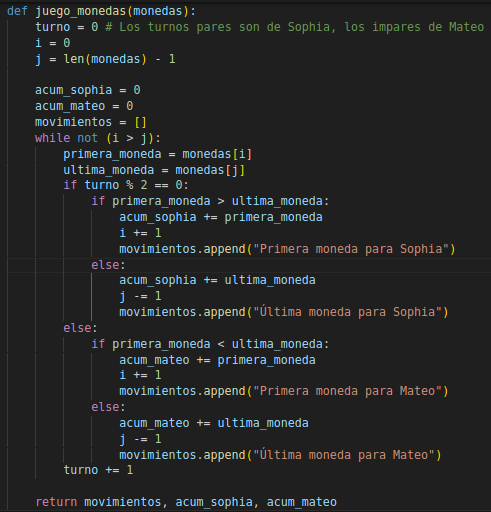
\includegraphics[scale = 0.75]{ {./images/algoritmo_codigo} }